\documentclass{article}
\usepackage{tikz}

\begin{document}

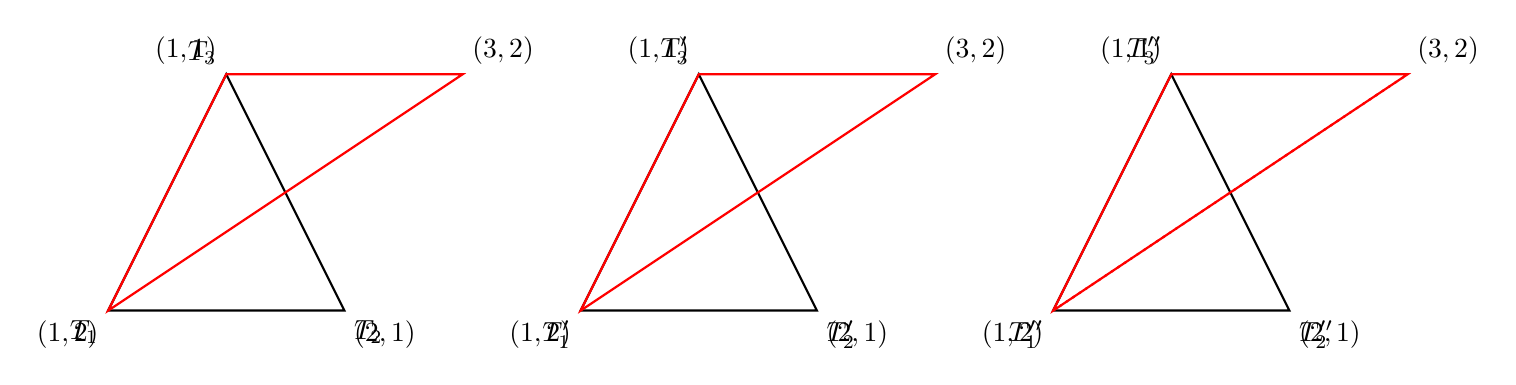
\begin{tikzpicture}[scale=1.5]
    % Define coordinates
    \coordinate (A) at (0,0);
    \coordinate (B) at (2,0);
    \coordinate (C) at (1,2);
    \coordinate (D) at (3,2);
    
    % Draw the main triangle
    \draw[thick] (A) -- (B) -- (C) -- cycle;
    
    % Label the vertices
    \node at (A) [below left] {$(1,2)$};
    \node at (B) [below right] {$(2,1)$};
    \node at (C) [above left] {$(1,1)$};
    \node at (D) [above right] {$(3,2)$};
    
    % Draw the smaller triangles
    \draw[red, thick] (A) -- (C) -- (D) -- cycle;
    \node at (A) [below left] {$T_{1}$};
    \node at (B) [below right] {$T_{2}$};
    \node at (C) [above left] {$T_{3}$};
    
    % Second set of coordinates
    \coordinate (A') at (4,0);
    \coordinate (B') at (6,0);
    \coordinate (C') at (5,2);
    \coordinate (D') at (7,2);
    
    % Draw the main triangle
    \draw[thick] (A') -- (B') -- (C') -- cycle;
    
    % Label the vertices
    \node at (A') [below left] {$(1,2)$};
    \node at (B') [below right] {$(2,1)$};
    \node at (C') [above left] {$(1,1)$};
    \node at (D') [above right] {$(3,2)$};
    
    % Draw the smaller triangles
    \draw[red, thick] (A') -- (C') -- (D') -- cycle;
    \node at (A') [below left] {$T'_{1}$};
    \node at (B') [below right] {$T'_{2}$};
    \node at (C') [above left] {$T'_{3}$};
    
    % Third set of coordinates
    \coordinate (A'') at (8,0);
    \coordinate (B'') at (10,0);
    \coordinate (C'') at (9,2);
    \coordinate (D'') at (11,2);
    
    % Draw the main triangle
    \draw[thick] (A'') -- (B'') -- (C'') -- cycle;
    
    % Label the vertices
    \node at (A'') [below left] {$(1,2)$};
    \node at (B'') [below right] {$(2,1)$};
    \node at (C'') [above left] {$(1,1)$};
    \node at (D'') [above right] {$(3,2)$};
    
    % Draw the smaller triangles
    \draw[red, thick] (A'') -- (C'') -- (D'') -- cycle;
    \node at (A'') [below left] {$T''_{1}$};
    \node at (B'') [below right] {$T''_{2}$};
    \node at (C'') [above left] {$T''_{3}$};
    
    % Dotted line for the third triangle
    \draw[dotted, red, thick] (A'') -- (D'');
    
    % Second dotted line for the third triangle
    \draw[dotted, red, thick] (C'') -- (D'');
\end{tikzpicture}

\end{document}